\section{Uniform and Non-Uniform Hierarchical B-Splines}
\label{sec:31standardBSplines}

\todo{add references}

In this section, we mainly follow the presentation of
\cite{Valentin14Hierarchische,Valentin16Hierarchical}
to define hierarchical B-splines.
Note that thanks to the groundwork laid in \cref{chap:20sparseGrids},
especially \thmref{lemma:tensorProductLinearIndependence} and
\thmref{prop:splittingUVToMV},
it completely suffices to study the univariate case
of all bases that will be defined in the rest of this thesis.
The multivariate case is treated as usual by the tensor product approach.



\subsection{Uniform Hierarchical B-Splines}

\todo{add references}

\paragraph{Cardinal B-splines}

\newgsymbol{bp}{$b^p$}{Cardinal B-spline of degree $p$}%
\newgsymbol{x01}{$\chi_A$}{Characteristic function of the set $A \subset \RR$}%
\newgsymbol{01!h}{$\halfopeninterval{\ß0, \ß1}$}{%
  Half-open unit interval $:= \halfopeninterval{0, 1}^d =
  \{x \in \RR \mid 0 \le x < 1\}^d$%
}%
The \term{cardinal B-spline}
$b^p\colon \RR \to \RR$ of \term{degree} $p \in \NN_0$
is defined by the recursion
\begin{equation}
  \label{eq:cardinalBSpline}
  b^p(x)
  :=
  \begin{cases}
    \displaystyle\int_0^1 b^{p-1}(x - y) \diff{}y,&p \ge 1,\\
    \chi_{\halfopeninterval{0, 1}}(x),&p = 0,
  \end{cases}
\end{equation}
where $\chi_{\halfopeninterval{0, 1}}$ is the characteristic function of
the half-open unit interval $\halfopeninterval{0, 1}$.
The cardinal B-spline $b^p$ has the following properties:
\begin{itemize}
  \item
  \newgsymbol{supp}{$\supp f$}{Support of a function $f$}%
  \emph{Support:}
  The support of $b^p$ is given by $\supp b^p = [0, p + 1]$.
  
  \item
  \emph{Bounds and symmetry:}
  The cardinal B-spline $b^p$ is non-negative and bounded from above by $1$.
  It is symmetric with respect to the center of its support, i.e.,
  $b^p(x) = b^p(p + 1 - x)$.
  
  \item
  \emph{Recursion:}
  The cardinal B-spline $b^p$ ($p \ge 1$) satisfies the following recurrence
  relation
  (which could be used as an alternative definition):
  \begin{equation}
    b^p(x)
    = \frac{x}{p} b^{p-1}(x) + \frac{p+1-x}{p} b^{p-1}(x-1).
  \end{equation}
  
  \item
  \emph{Spline:}
  On every \term{knot interval} $\halfopeninterval{k, k+1}$
  ($k = 0, \dotsc, p$), $b^p$ is a polynomial of degree~$p$, i.e.,
  $b^p$ is a spline (piecewise polynomial).
  
  \item
  \emph{Differentiability:}
  At the \term{knots} $k = 0, \dotsc, p + 1$,
  $b^p$ is $(p - 1)$ times continuously differentiable.
  The derivative can be computed by differentiating
  \eqref{eq:cardinalBSpline}:
  \begin{equation}
    \label{eq:cardinalBSplineDerivative}
    \frac{\diff}{\dx} b^p(x)
    = b^{p-1}(x) - b^{p-1}(x-1),\quad
    x \in \RR.
  \end{equation}
  
  \item
  \emph{Convolution:}
  The integral in the definition of $b^p$
  is the convolution $b^{p-1} \ast b^0$ of the B-spline $b^{p-1}$
  of degree $p - 1$ with the B-spline $b^0$ of degree $0$.
  
  \item
  \emph{Generalization:}
  \newgsymbol{dij}{$\delta_{i,j}$}{%
    Kronecker delta $:= 1$ if $i = j$ and $:= 0$ otherwise%
  }%
  As a special case, $b^1$ is a hat function interpolating the data
  $\{(k, \delta_{k,1}) \mid k \in \ZZ\}$.
  One can show that for the limit of $p \to \infty$,
  $b^p$ converges to the Gaussian bell curve function
  $b^\infty(x) := (2\pi)^{-1/2} \exp(-x^2/2)$.
  \todo{check, more exact}
\end{itemize}
The cardinal B-splines of the first degrees are shown in
\cref{fig:cardinalBSpline}.
Due to the convolution property,
which is visualized with the flip book animation in the bottom left corner
of the pages of this thesis,
cardinal B-splines of degree $p \ge 2$ are ``smoothed versions''
of the hat function.

\begin{figure}
  \includegraphics{cardinalBSpline_1}%
  \caption{Cardinal B-splines $b^p$ up to quintic degree $p = 5$.}%
  \label{fig:cardinalBSpline}
\end{figure}

\paragraph{Uniform hierarchical B-splines}

\newgsymbol{.p}{$\cdot^p$}{%
  Superscript for ``B-spline (basis function/function space/interpolant)
  of degree $p$''%
}%
We can use the cardinal B-spline $b^p$ as a ``mother function'' to
define the uniform hierarchical B-spline
$\varphi_{l,i}^p\colon [0, 1] \to \RR$ of level $l \in \NN_0$ and index
$i \in I_l$ via an affine parameter transformation:
\todo{citation [28] in SGA?}
\begin{equation}
  \label{eq:uniformHierarchicalBSplineUV}
  \varphi_{l,i}^p(x)
  := b^p(x/h_l + (p+1)/2 - i).
\end{equation}
The support of $\varphi_{l,i}^p$ is given
by $\supp \varphi_{l,i}^p = [0, 1] \cap (h_l \cdot [i \pm (p+1)/2])$,
where $[i \pm (p+1)/2] := [i - (p+1)/2, i + (p+1)/2]$.
The hat function basis $\varphi_{l,i}^1$ defined in
\eqref{eq:hatFunctionUV} is a special case of
\eqref{eq:uniformHierarchicalBSplineUV} for $p = 1$,
which allows us to use the same notation $\varphi_{l,i}^p$ for both.
Note that due to the \term{translation invariance} of $\varphi_{l,i}^p$
(i.e., the basis functions are the same up to scaling and translation),
it suffices to precompute and implement the polynomial pieces of $b^p$
to enable evaluations of all hierarchical B-splines
$\varphi_{l,i}^p$, $l \in \NN_0$, $i \in I_l$.

\begin{figure}
  \subcaptionbox{%
    Nodal B-splines $\varphi_{l,i}^p$ ($i \in I_l$) and grid points $x_{l,i}$
    \emph{(dots)}.%
  }[70mm]{%
    \includegraphics{hierarchicalBSpline_1}%
  }%
  \hfill%
  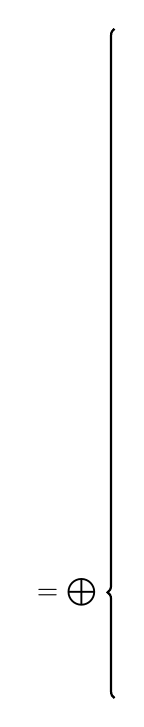
\begin{tikzpicture}
    \draw[decorate,thick,decoration={brace,aspect=0.158}] (0,-8.5) -- (0,0);
    \node[anchor=east] at (-0.1,-7.157) {$= \bigoplus$};
  \end{tikzpicture}%
  \hfill%
  \subcaptionbox{%
    Hierarchical B-splines $\varphi_{l',i'}^p$ ($l' \le l$, $i' \in I_{l'}$)
    and grid points $x_{l',i'}$
    \emph{(dots)}.%
  }[72mm]{%
    \includegraphics{hierarchicalBSpline_2}%
  }%
  \caption{%
    Univariate nodal and hierarchical cubic B-splines ($p = 3$)
    up to level $l = 3$.
    When restricting all functions to $D_l^p$ \emph{(thick black line)},
    the nodal space $V_l^p|_{D_l^p}$ decomposes into the direct sum
    of the hierarchical subspaces $W_{l'}^p|_{D_l^p}$ ($l' \le l$).%
  }
  \label{fig:hierarchicalBSpline}
\end{figure}

\paragraph{Odd and even degrees}

In the following, we will only allow odd degrees $p = 1, 3, 5, \dotsc$
in this thesis.
Many theoretical considerations would fail for even degrees.
The basic reason is that for odd degrees, the knots of
$\varphi_{l,i}^p$ coincide with the grid points
\begin{equation}
  x_{l,i-(p+1)/2},\quad
  \dotsc,\quad
  x_{l,i},\quad
  \dotsc,\quad
  x_{l,i+(p+1)/2}.
\end{equation}
For even degrees $p$, the knots of $\varphi_{l,i}^p$ lie exactly in
the middle between two subsequent grid points:
\begin{equation}
  x_{l,i-p/2} - \frac{h_l}{2},\quad
  \dotsc,\quad
  x_{l,i} - \frac{h_l}{2},\quad
  x_{l,i} + \frac{h_l}{2},\quad
  \dotsc,\quad
  x_{l,i+p/2} + \frac{h_l}{2}.
\end{equation}
As we will see in this thesis,
this fact would have many adverse implications.
Most crucial among these are
that the hierarchical splitting \eqref{eq:hierSplittingUV} would not hold,
\todo{insert reference}
that non-uniform hierarchical B-splines would not be able to be defined as
simple as for odd degree,
\todo{insert reference} and
that the so-called fundamental splines would not be defined at all.
\todo{insert reference}
Therefore, and
as these degrees include the hat function case ($p = 1$) and the
most common applied cubic degree ($p = 3$),
it is reasonable to restrict ourselves to odd degrees
for the rest of the thesis.



\subsection{Non-Uniform B-Splines and Proof of the Hierarchical Splitting}

\paragraph{Non-uniform B-splines and spline space}

With the hierarchical B-splines $\varphi_{l,i}^p$, we can define
the nodal spaces $V_l^p$ and hierarchical subspaces $W_l^p$
as in \cref{chap:20sparseGrids}.
However, in order for the hierarchical splitting \eqref{eq:hierSplittingUV}
to be correct, we have to prove that the conditions of
\thmref{lemma:hierSplittingUV} are satisfied.
To investigate how the nodal space $V_l^p$ looks like,
we introduce the notion of non-uniform B-splines.

\begin{definition}[non-uniform B-splines]
  \label{def:nonUniformBSpline}
  \newgsymbol{xi!}{$\ß\xi$}{%
    Knot sequence $:= (\xi_0, \dotsc, \xi_{m+p})$%
  }%
  Let $m, p \in \NN_0$ and $\ß\xi = (\xi_0, \dotsc, \xi_{m+p})$ be an
  increasing sequence of real numbers \term{(knot sequence)}.
  \newgsymbol{bkxip}{$b_{k,\ß\xi}^p$}{%
    Non-uniform B-spline of degree $p$ with knots $\ß\xi$ and index $k$%
  }%
  For $k = 0, \dotsc, m - 1$,
  the \term{(non-uniform) B-spline} $b_{k,\ß\xi}^p$ of degree $p$
  with knots $\ß\xi$ and index $k$ is defined by the
  Cox--de Boor recurrence
  \cite{Cox72Numerical,Boor72Calculating,Hoellig13Approximation}
  \begin{equation}
    b_{k,\ß\xi}^p(x)
    :=
    \begin{cases}
      \dfrac{x - \xi_k}{\xi_{k+p} - \xi_k} b_{k,\ß\xi}^{p-1}(x) +
      \dfrac{\xi_{k+p+1} - x}{\xi_{k+p+1} - \xi_{k+1}}
      b_{k+1,\ß\xi}^{p-1}(x),&p \ge 1,\\
      \chi_{\halfopeninterval{\xi_k, \xi_{k+1}}}(x),&p = 0.
    \end{cases}
  \end{equation}
\end{definition}
Note that when choosing $\ß\xi = (0, 1, \dotsc, p + 1)$ and
$k = 0$, we obtain the cardinal B-spline $b^p$.
The definition can be used to characterize the nodal space $V_l^p$:

\begin{proposition}[spline space]
  \label{prop:splineSpace}
  \newgsymbol{Sxip}{$S_\ß\xi^p$}{%
    Spline space of degree $p$ with knots $\ß\xi$%
  }%
  Let $\ß\xi = (\xi_0, \dotsc, \xi_{m+p})$ be a knot sequence.
  Then, the B-splines $b_{k,\ß\xi}^p$ ($k = 0, \dotsc, m - 1$)
  form a basis of the \term{spline space}
  \begin{equation}
    S_\ß\xi^p
    := \spn\{b_{k,\ß\xi}^p \mid k = 0, \dotsc, m - 1\}.
  \end{equation}
  $S_\ß\xi^p$ contains exactly those functions which are continuous
  on $D_\ß\xi^p := [\xi_p, \xi_m]$,
  polynomials of degree $\le p$ on every knot interval
  $[\xi_k, \xi_{k+1}]$ \todo{check half-open interval?} in $D_\ß\xi$
  ($k = p, \dotsc, m - 1$) and at least $(p - 1)$ times
  continuously differentiable at every knot $\xi_k$ in the interior of
  $D_\ß\xi^p$ ($k = p + 1, \dotsc, m - 1$).
\end{proposition}

\begin{proof}
  See \cite{Hoellig13Approximation}.
\end{proof}

This proposition gives the reason for ``B'' in ``B-splines'',
which is for ``basis'' (of the space of splines).
The key observation is that B-splines of a knot sequence $\ß\xi$
do not form a basis of the spline space on the union
$[\xi_0, \xi_{m+p}]$ of the B-spline supports,
but rather on a proper sub-interval $D_\ß\xi^p$.
Intuitively, for every point in $D_\ß\xi^p$ that is not a knot,
exactly $(p + 1)$ B-splines must be \term{relevant} (i.e., non-zero)
to span the spline space as
on every knot interval, the spline is a polynomial of degree $\le p$
and therefore, there must be $(p + 1)$ degrees of freedom.
Outside of $D_\ß\xi^p$, there are too few relevant B-splines
to span the spline space.
This important observation, which is visualized in \cref{fig:splineSpace},
forces us to restrict nodal space and hierarchical subspaces to
$D_\ß\xi^p$:

\begin{figure}
  \includegraphics{splineSpace_1}%
  \caption{%
    Knot sequence $\ß\xi = (\xi_0, \dotsc, \xi_{m+p}$)
    with the corresponding $m = 7$ non-uniform cubic B-splines
    $b_{k,\ß\xi}^p$, $k = 0, \dotsc, m - 1$, $p = 3$.
    On $D_\ß\xi^p$ \emph{(thick line, delimited by dashed lines)},
    which starts with the last knot interval of the first B-spline
    $b_{0,\ß\xi}^p$
    and ends with the first knot interval of the last B-spline
    $b_{m-1,\ß\xi}^p$,
    the B-splines span the spline space $S_\ß\xi^p$.
    \newgsymbol{s}{$s$}{Spline (piecewise polynomial)}%
    Elements of this space are splines $s\colon D_\ß\xi^p \to \RR$
    \emph{(black line)},
    which are linear combinations
    $s = \sum_{k=0}^{m-1} c_k b_{k,\ß\xi}^p$
    of the B-splines.%
  }%
  \label{fig:splineSpace}
\end{figure}

\begin{corollary}[nodal B-spline space]
  \label{cor:nodalBSplineSpace}
  \newgsymbol{f|D}{$f|_D$}{%
    Restriction $f|_D\colon D \to \RR$, $f|_D(x) := f(x)$,
    onto a sub-domain $D$ for a function $f$%
  }%
  \newgsymbol{V|D}{$V|_D$}{%
    Restriction $:= \{f|_D \mid f \in V\}$ onto a sub-domain $D$
    for a function space $V$%
  }%
  \newgsymbol{xilp}{$\ß\xi_l^p$}{%
    Knot sequence
    for uniform nodal B-splines of level $l$, degree $p$%
  }%
  \newgsymbol{Slp}{$S_l^p$}{%
    Spline space $:= S_{\ß\xi_l^p}^p$
    (spanned by the uniform nodal B-splines of level $l$, degree $p$)%
  }%
  \newgsymbol{Dlp}{$D_l^p$}{%
    Spline interpolation domain of $S_l^p$
    (uniform nodal B-splines of level $l$, degree $p$)%
  }%
  The restricted nodal B-splines $\varphi_{l,i}^p|_{D_l^p}$
  ($i = 0, \dotsc, 2^l$)
  of level $l \in \NN_0$ are
  a basis of the spline space $S_{\ß\xi_l^p}^p$, where
  \begin{gather}
    \label{eq:nodalBSplineSpaceKnots}
    \xi_{l,k}^p
    := (k - (p+1)/2) h_l,\quad
    k = 0, \dotsc, m + p,\quad
    m := 2^l + 1,\\
    D_l^p := \left[h_l \frac{p-1}{2},\; 1 - h_l \frac{p-1}{2}\right],
  \end{gather}
  and consequently
  \begin{equation}
    V_l^p|_{D_l^p}
    = S_l^p
    := S_{\ß\xi_l^p}^p.
  \end{equation}
\end{corollary}

\begin{proof}
  We have $\varphi_{l,i}^p = b_{i,\ß\xi_l^p}^p$ for
  $i = 0, \dotsc, m - 1$,
  as the B-splines on both sides have the same knots.
  The assertions now follow from \thmref{prop:splineSpace}.
\end{proof}

Note that $D_l^p$ might contain only a single point or even be empty,
if $p$ is too large or $l$ is too small.
However, the corresponding B-splines $\varphi_{l,i}^p$ are still linearly
independent on $[0, 1]$ (see \cite{Hoellig13Approximation}).
Similarly, the corollary also implies that the hierarchical functions
$\varphi_{l,i}^p$ ($i \in I_l$) are linearly independent on $[0, 1]$.

\paragraph{Hierarchical splitting for uniform B-splines}

We can use \cref{prop:splineSpace} and \cref{cor:nodalBSplineSpace}
to prove the hierarchical splitting for the uniform B-spline basis.

\begin{lemma}[first condition of \cref{lemma:hierSplittingUV}]
  The restricted hierarchical subspaces
  $W_{l'}^p|_{D_l^p}$ ($l' \le l$) are
  subspaces of the restricted nodal space $V_l^p|_{D_l^p}$.
\end{lemma}

\begin{proof}
  Every function $\varphi_{l',i'}^p$ ($i' \in I_{l'}$) is continuous on
  $D_l^p$, a polynomial of degree $\le p$ on every knot interval
  of $\ß\xi_l^p$ (due to $p$ odd),
  and at the knots themselves at least $(p - 1)$ times continuously
  differentiable.
  \Cref{prop:splineSpace} implies $\varphi_{l',i'}^p \in S_l^p$
  and from \cref{cor:nodalBSplineSpace}, it follows
  $\varphi_{l',i'}^p \in V_l^p|_{D_l^p}$.
  As the functions $\varphi_{l',i'}^p$ ($i' \in I_{l'}$) span
  $W_{l'}^p|_{D_l^p}$, we can conclude
  $W_{l'}^p|_{D_l^p} \subset V_l^p|_{D_l^p}$.
\end{proof}

It is crucial to note that this lemma does not hold for even $p$,
as the knots of the B-splines of level $l - 1$ are not contained in the
knots of level $l$.
This implies that in general,
$W_{l-1}^p|_{D_l^p}$ is not contained in $V_l^p|_{D_l^p}$
for even degrees $p$.
Therefore, the hierarchical splitting equation \eqref{eq:hierSplittingUV}
does not hold, which is the reason for us to restrict the
remaining considerations to odd $p$.

\begin{restatable}[second condition of \cref{lemma:hierSplittingUV}]{%
  proposition%
}{%
  propHierBSplineLinearlyIndependent%
}
  \label{prop:hierBSplineLinearlyIndependent}
  \label{PROP:HIERBSPLINELINEARLYINDEPENDENT}
  The hierarchical B-splines
  $\varphi_{l',i'}^p$ ($l' \le l$, $i' \in I_{l'}$)
  are linearly independent.
\end{restatable}

\begin{proof}
  See \cref{sec:proofHierBSplineLinearlyIndependent}.
\end{proof}

Although we have to restrict all functions and spaces to $D_l^p$,
\thmref{lemma:hierSplittingUV} is still applicable to prove that
the hierarchical splitting equation \eqref{eq:hierSplittingUV}
is correct for hierarchical B-splines:

\begin{corollary}[hierarchical splitting for uniform B-splines]
  \label{cor:hierSplittingBSpline}
  The hierarchical splitting \eqref{eq:hierSplittingUV}
  holds for the hierarchical B-spline basis
  if restricting all functions to $D_l^p$:
  \begin{equation}
    S_l^p
    = V_l^p|_{D_l^p}
    = \bigoplus_{l'=0}^l W_{l'}^p|_{D_l^p}.
  \end{equation}
\end{corollary}

\begin{proof}
  Analogously to the proof of \thmref{lemma:hierSplittingUV}
  and apply \thmref{cor:nodalBSplineSpace}.
\end{proof}

This corollary is also visualized in \cref{fig:hierarchicalBSpline}.
We can now proceed to define multivariate
nodal spaces $V_\ßl^p$, hierarchical subspaces $W_\ßl^p$, and
sparse grid spaces $V_{n,d}^{\sparse,p}$ as in \cref{chap:20sparseGrids}.
Note that it is possible to choose different degrees $p_t$ for
different dimensions $t = 1, \dotsc, d$,
since the hierarchical splitting \eqref{eq:hierSplittingMV} does not
require the bases in each dimension to be the same.
Consequently, we can define degree-dimension-adaptive sparse grids
$V_{n,d}^{\sparse,\ßp}$ for arbitrary odd degree vectors $\ßp$.

In the course of this thesis, we will derive multiple variations
of the standard hierarchical B-spline basis.
We will not repeat formal proofs of the hierarchical splitting equation
\eqref{eq:hierSplittingUV}
(i.e., verifying the two conditions of \cref{lemma:hierSplittingUV})
for each of theses bases for the sake of brevity.
The idea of the proof of \cref{prop:hierBSplineLinearlyIndependent},
which is inductively exploiting the smoothness conditions given by
B-splines of previous levels, can often be transferred to similar B-spline
bases.



\subsection{Modification}

\paragraph{Marsden's identity}

Similarly to the piecewise linear case in \cref{sec:24boundary},
Pflüger defined modified
hierarchical B-splines to obtain reasonable values on the boundary
without having to place grid points there \cite{Pflueger10Spatially}.
In \cite{Pflueger10Spatially}, the main motivation is to define basis
functions $\varphi_{l,i}^{p,\modified}$ that satisfy natural boundary
conditions, i.e.,
\begin{equation}
  \label{eq:naturalBoundaryConditions}
  \frac{\diff^2}{\dx^2} \varphi_{l,i}^{p,\modified}(x) = 0,\quad
  x \in \bndry{[0, 1]} = \{0, 1\}.
\end{equation}
Originally, this requirement stems from financial problems
\cite{Pflueger10Spatially}.

For the left boundary,
\eqref{eq:naturalBoundaryConditions} can be satisfied by
modifying the left-most function $\varphi_{l,1}^p$ such that
$\varphi_{l,1}^{p,\modified}(x) = 2 - x/h_l$ is a linear polynomial
when $x$ is ``near'' the boundary.
As in \cite{Pflueger10Spatially},
we append $\varphi_{l,1}^p$ with
B-splines $\varphi_{l,i}^p$ with index $i \le 0$ and
use the so-called Marsden's identity to compute the corresponding
coefficients:

\begin{lemma}[Marsden's identity]
  \label{lemma:marsden}
  Let $p \in \NN_0$ and
  $\ß\xi = (\xi_0, \dotsc, \xi_{m+p})$ be a knot sequence.
  Then, for all $x \in D_\ß\xi^p$ and $y \in \RR$,
  \begin{equation}
    \label{eq:marsden}
    (x - y)^p
    = \sum_{k=0}^{m-1} \big[(\xi_{k+1} - y) \dotsm (\xi_{k+p} - y)\big]
    b_{k,\ß\xi}^p(x).
  \end{equation}
\end{lemma}

\begin{proof}
  See \cite{Hoellig13Approximation}.
\end{proof}

\paragraph{Modified hierarchical B-splines}

By applying Marsden's identity twice,
\begin{equation}
  2 - \frac{x}{h_l}
  = 2 \sum_{i \in \ZZ} \varphi_{l,i}^p(x)
  - \frac{1}{h_l} \sum_{i \in \ZZ} x_{l,i} \varphi_{l,i}^p(x)
  = \sum_{i \in \ZZ} (2 - i) \varphi_{l,i}^p(x),\quad
  x \in \RR,
\end{equation}
we obtain a possible definition for $\varphi_{l,i}^{p,\modified}$.
Note that only the B-splines with $i \ge 1 - (p+1)/2$
are relevant for the unit interval as all other B-splines vanish in $[0, 1]$.
Pflüger omits summands with $i > 1$ as he only wants to modify
$\varphi_{l,1}^p$ left of its grid point $x_{l,1}$.
The right-most function $\varphi_{l,2^l-1}^{p,\modified}$ can be derived
analogously by mirroring $\varphi_{l,1}^{p,\modified}$ at $0.5$.
For $l = 1$, again the ``constant $1$'' function is taken for the definition
of modified hierarchical B-splines (see \cref{fig:modifiedBSpline}):
\begin{equation}
  \label{eq:modifiedBSpline}
  \varphi_{l,i}^{p,\modified}(x)
  :=
  \begin{cases}
    1,&
    l = 1,\quad i = 1,\\
    \displaystyle\sum_{i'=1-(p+1)/2}^1 (2 - i') \varphi_{l,i'}^p(x),&
    l \ge 2,\quad i = 1,\\
    \varphi_{l,i}^p(x),&
    l \ge 2,\quad i \in I_l \setminus \{1, 2^l - 1\},\\
    \varphi_{l,1}^{p,\modified}(1 - x),&
    l \ge 2,\quad i = 2^l - 1.
  \end{cases}
\end{equation}
By \thmref{prop:splineSpace},
this definition implies that
$\varphi_{l,1}^p(x) = 2 - x/h_l$ ($l \ge 2$)
is only valid for $x \in [0,\; h_l \cdot (5-p)/2]$, i.e.,
the second derivative at $x = 0$ vanishes only for $p \le 5$.
For higher degrees, it is non-zero, albeit very small
in its absolute value.
If it is desired to enforce natural boundary conditions
for higher than quintic degrees,
then the upper bound of $i'$ in the sum in \eqref{eq:modifiedBSpline}
must be extended to $(p+1)/2 - 1$.

\begin{figure}
  \subcaptionbox{%
    Construction of the modified hierarchical cubic B-spline
    $\varphi_{l,1}^{p,\modified}$ (\emph{dashed}, $l \ge 2$)
    as a linear combination of neighboring B-splines $\varphi_{l,i'}^p$
    using Marsden's identity.%
  }[75mm]{%
    \includegraphics{modifiedBSpline_1}%
  }%
  \hfill%
  \subcaptionbox{%
    Modified hierarchical cubic B-splines $\varphi_{l,i}^{p,\modified}$
    and grid points $x_{l,i}$
    \emph{(dots)}.%
  }[75mm]{%
    \includegraphics{hierarchicalBSpline_3}%
  }%
  \caption{%
    Construction of modified hierarchical B-splines and
    the resulting basis.%
  }
  \label{fig:modifiedBSpline}
\end{figure}



\subsection{Non-Uniform Hierarchical B-Splines}

Sparse grid spaces and their corresponding grid point sets,
as we have defined them in \cref{chap:20sparseGrids},
are completely independent of the actual location of the grid points
$x_{l,i}$.
Therefore, it is possible to use different distributions for the grid points
than the standard equidistant choice of $x_{l,i} = i \cdot h_l$,
if the basis functions are altered accordingly.
The so-called Chebyshev points $x_{l,i}^\clenshawcurtis$ and the
resulting Clenshaw--Curtis grids and B-splines will serve as an example.

\paragraph{Chebyshev points and Clenshaw--Curtis grids}

\newgsymbol{.cc}{$\cdot^\clenshawcurtis$}{%
  Superscript for ``Clenshaw--Curtis (grid point/grid point set/basis
  function/function space/interpolant)''%
}%
The \term{Chebyshev points} $x_{l,i}^\clenshawcurtis$ of level $l \in \NN_0$
are defined as
\begin{equation}
  x_{l,i}^\clenshawcurtis
  := \frac{1 - \cos(\pi x_{l,i})}{2},\quad
  i = 0, \dotsc, 2^l.
\end{equation}
Chebyshev points are the normalized locations of the extrema of the
Chebyshev polynomials $T_{2^l}\colon [-1, 1] \to \RR$,
$T_{2^l}(x) := \cos(2^l \arccos(x))$ \cite{Xu16Chebyshev}.%
\footnote{%
  The literature sometimes uses the name ``Chebyshev points'' for
  the roots of $T_{2^l}$, which are closely connected to the extrema.
  One way to distinguish them is to call the extrema
  ``Chebyshev--Lobatto points'' and the roots
  ``Chebyshev--Gauss points'' \cite{Xu16Chebyshev}.%
}
They are obtained by dividing a semicircle into $2^l$ equally sized
segments and subsequently orthogonally projecting the
segment endpoints onto the diameter
(see \cref{fig:chebyshev}).
The most practical use of Chebyshev points is for
polynomial interpolation to avoid Runge's phenomenon and for
so-called Clenshaw--Curtis quadrature rules.

\begin{figure}
  \includegraphics{chebyshev_1}%
  \caption{%
    Chebyshev points $x_{l,i}^\clenshawcurtis$ on the unit interval $[0, 1]$
    \emph{(black lines)}
    for $l = 0, \dotsc, 4$
    and their construction as the orthogonal projection of the
    endpoints of $2^l$ equally sized segments
    of a semicircle onto its diameter \emph{\textcolor{C0}{(blue)}}.%
  }
  \label{fig:chebyshev}
\end{figure}

In some settings, it can be beneficial to use full or sparse grids consisting
of Chebyshev points, which are then called \term{Clenshaw--Curtis grids},
instead of uniform grids.
Besides the already mentioned advantages for polynomial integration and
quadrature, Clenshaw--Curtis grids can help to reduce interpolation
error in a neighborhood of the boundary of the domain due to the increased
grid point density near the boundary.
If we want to use Chebyshev points as grid points for sparse grids,
we have to employ an appropriate basis to ensure that interpolation
is still possible.
Fortunately, \cref{def:nonUniformBSpline} specifies B-splines for non-uniform
knot sequences.

\paragraph{Hierarchical Clenshaw--Curtis B-splines}

The \term{hierarchical Clenshaw--Curtis B-spline}
$\varphi_{l,i}^{p,\clenshawcurtis}$ of level $l \in \NN_0$ and index
$i \in I_l$ is defined as
\begin{equation}
  \varphi_{l,i}^{p,\clenshawcurtis}
  := b_{i,\ß\xi_l^{p,\clenshawcurtis}}^p,
\end{equation}
where
\begin{subequations}
  \label{eq:clenshawCurtisBSplineKnots}
  \begin{gather}
    \xi_{l,k}^{p,\clenshawcurtis}
    :=
    \begin{cases}
      (k - \frac{p+1}{2}) \cdot x_{l,1}^\clenshawcurtis,&
      k = 0, \dotsc, \frac{p-1}{2},\\
      x_{l,k-(p+1)/2}^\clenshawcurtis,&
      k = \frac{p+1}{2}, \dotsc, 2^l + \frac{p+1}{2},\\
      1 + (k - 2^l - \frac{p+1}{2}) \cdot x_{l,1}^\clenshawcurtis,&
      k = 2^l + \frac{p+3}{2}, \dotsc, 2^l + p + 1,
    \end{cases}\\
    k = 0, \dotsc, m + p,\quad
    m := 2^l + 1.
  \end{gather}
\end{subequations}
For the construction of the knot sequence $\ß\xi_l^{p,\clenshawcurtis}$,
the Chebyshev points $x_{l,i}^\clenshawcurtis$
are equidistantly extended onto the real line $\RR$.
As for the standard hierarchical B-spline basis,
it is now straightforward to define nodal spaces
$V_l^{p,\clenshawcurtis}$
and hierarchical subspaces $W_l^{p,\clenshawcurtis}$ as well as
sparse grid spaces $V_{n,d}^{\sparse,p,\clenshawcurtis}$ and
grid point sets $\Omega_{n,d}^{\sparse,\clenshawcurtis}$
using Cartesian products of Chebyshev points
and tensor products of Clenshaw--Curtis B-splines.
The one-dimensional cubic Clenshaw--Curtis basis and a two-dimensional
sparse Clenshaw--Curtis grid are shown in \cref{fig:clenshawCurtis}.

\begin{figure}
  \subcaptionbox{%
    Hierarchical cubic Clenshaw--Curtis B-splines
    $\varphi_{l,i}^{p,\clenshawcurtis}$ and
    modified Clenshaw--Curtis B-splines
     $\varphi_{l,i}^{p,\clenshawcurtis,\modified}$
    \emph{(dashed)}.%
  }[75mm]{%
    \includegraphics{hierarchicalBSpline_4}%
  }%
  \hfill%
  \subcaptionbox{%
    Sparse Clenshaw--Curtis grid $\Omega_{n,d}^{\sparse,\clenshawcurtis}$
    of level $n = 4$ in $d = 2$ dimensions.%
  }[75mm]{%
    \includegraphics{sg_7}%
  }%
  \caption{%
    Clenshaw--Curtis B-splines and sparse grids.%
  }
  \label{fig:clenshawCurtis}
\end{figure}

Note that in contrast to the standard hierarchical B-spline functions
$\varphi_{l,i}^p$, the Clenshaw--Curtis functions
$\varphi_{l,i}^{p,\clenshawcurtis}$ are not translation-invariant.
As a result, both implementation effort and evaluation runtime
are significantly higher for Clenshaw--Curtis B-splines than
for the standard uniform basis,
as the Clenshaw--Curtis B-splines cannot be precomputed.

\paragraph{Modification and generalizations}

Like for uniform B-splines,
\term{modified hierarchical Clenshaw--Curtis B-splines}
$\varphi_{l,i}^{p,\clenshawcurtis,\modified}$ can be defined using the
same method as in \eqref{eq:modifiedBSpline}.
Here, the second derivative does not vanish exactly at the boundary
even for degrees $p \le 5$,
as the formula derived from \thmref{lemma:marsden} assumes uniform knots.
However, as most of the B-spline knots in the summation formula
lie outside $[0, 1]$ and are thus uniformly extended according
to \eqref{eq:clenshawCurtisBSplineKnots},
the absolute deviation of the second derivative from $0$ is small.
Again, to enforce the natural boundary condition,
it is possible to recompute the coefficients
of the components $\varphi_{l,i'}^{p,\clenshawcurtis}$
dynamically with Marsden's identity using the correct Chebyshev knots
in \eqref{eq:marsden}.

Please note that our framework permits arbitrary grid point distributions
$x_{l,i}^\ast$,
as long as their number grows exponentially
(i.e., there are $2^l + 1$ points $x_{l,i}^\ast$ in each level $l \in \NN_0$)
and they are nested
(i.e., \eqref{eq:rewriteGridPoint} holds).
Appropriate non-uniform B-spline bases could be defined analogously
to Clenshaw--Curtis B-splines.
